\documentclass{article}
\usepackage{amsmath,amsthm,amssymb}
\usepackage{hyperref}
\usepackage{mathtools}
\DeclarePairedDelimiter\norm{\lVert}{\rVert}
\DeclarePairedDelimiter\abs{\lvert}{\rvert}
\DeclarePairedDelimiter\inner{\langle}{\rangle}
\def\emptyset{\varnothing}
\def\QEDclosed{\mbox{\rule[0pt]{1.3ex}{1.3ex}}}%hacked from IEEEtran.cls
\def\proofname{\normalfont \bfseries Proof}
\renewcommand\qedsymbol{\QEDclosed}
% resolve formula numbering
% all styles are plain, which is not optimal
% the official amsthm doc said we should use <definition> style for Definition,Example and Exercise.
\newtheorem{example}{Example}[section] % parent counter setting
\newtheorem{definition}{Definition}[section]
\newtheorem{exercise}{Exercise}[section]
\newtheorem{lemma}{Lemma}[section]
\newtheorem{remark}{Remark}[section]
\usepackage{xpatch}%remove the dot after theorem env
\makeatletter
\AtBeginDocument{\xpatchcmd{\@thm}{\thm@headpunct{.}}{\thm@headpunct{}}{}{}}
\makeatother
\usepackage{enumitem}
\begin{document}
% 
\title{Lecture 2 remark: Separation axioms and Countabilities (page 1 finished)}
\author{zhaofeng-shu33}
\maketitle
\section{Topological space: separation axioms}

\begin{figure}[!ht]
\centering
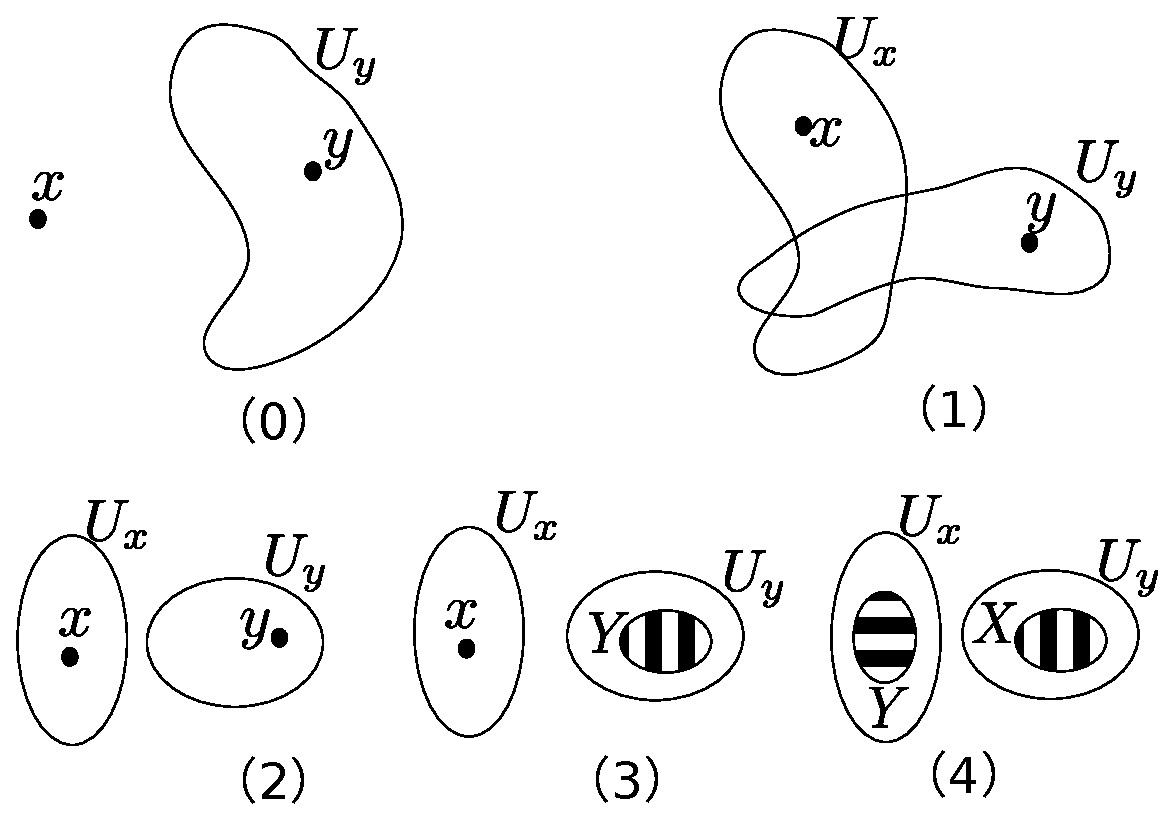
\includegraphics[width=\textwidth]{T04.eps}
\caption{Illustrations on $T_0$ to $T_4$}
\end{figure}
\setcounter{example}{0}
\begin{example}
Let $X=\{a,b\},T=\{\emptyset,X,\{a\}\}$, Then $T$ satisfies $T_0$, but does not satisfy $T_1$.
\end{example}
\begin{example}[Lecture 1 remark \normalfont{\textbf{Example 1.4}} continued]
$T$ satisfies $T_1$, but does not satisfy $T_2$ (Notice for $x\neq y, \mathbb{R}\backslash\{x\}\ni y,\not\owns x; \mathbb{R}\backslash\{y\} \ni x,\not\owns y$, thus satisfying $T_1$).
\end{example}
\begin{example}
If $x\notin Y$, where $Y$ is closed, then $d(x,Y)=\inf\{d(x,y)|y\in Y\}>0$.
\begin{proof}
Suppose $d(x,Y)=0$. By the definition of inferior of number set, we can find $\{y_n\}$ such that $d(x,y_n)\to 0$.
For any neightborhood $V$ of $x$, we can find $B(x,r)\subseteq V$. For sufficient large $n,y_n \in B(x,r) \Rightarrow V$ contains point in $Y\backslash{x}$.
By the definition of accumulated point of $Y$, $x\in Y'$. Since $Y$ is closed, if $x \in Y^c$, which is open, we can find $U$ such that $x\in U\subseteq Y^c$, which contradicts with the fact that $x$ is the accumulated point of $Y$. Therefore, $x\in Y$, which contradicts $x\notin Y$.
\end{proof}
\end{example}
\setcounter{lemma}{3}
\begin{lemma}
A metric space $X$ is Hausdorff ($T_2$), and $x_n\to x, x_n\to y$, then $x=y$.
\begin{proof}
Suppose $x\neq y$, then there exists disjoint open set $U,V$ s.t. $x\in U,y\in V$. Then by the definition of convergence, both $U$ and $V$ contain almost $\{x_n\}$, a contradiction.  
\end{proof}
\end{lemma}
\setcounter{lemma}{5}
\begin{lemma}\mbox{}
\begin{enumerate}[label=(\alph*)]
\item $(X,T)$ is $T_3$ if and only if for any $x\in X$ and an open neighborhood $U$ of $x$, there exists an open set $V$, such that $x\in V\subseteq \bar{V}\subseteq U$
\item $(X,T)$ is $T_4$ if and only if for any closed set $A$ and an open neighborhood $U$\reflectbox{$\subseteq$} $A$, there exists an open set $V$, such that $A\subseteq V\subseteq \bar{V}\subseteq U$
\end{enumerate}
\begin{proof}\mbox{}
\begin{enumerate}[label=(\alph*)]
\item $\Rightarrow$ $U^c$ is closed, and $x\notin U^c$. Then by $T_3$ property, there exists an open set $V_1\ni x$, another open set $V_2$ \reflectbox{$\subseteq$} $U^c$ and $V_1\cap V_2 =\emptyset$. Then it follows that $V_1\subseteq U$. Also $\bar{V}_1 \cap V_2 = \emptyset \Rightarrow \bar{V}_1 \subseteq U$. Therefore, choose $V=V_1$ and $x\in V\subseteq \bar{V}\subseteq U$.

$\Leftarrow$ Given $x$ and a closed set $A$, $x\notin A$, then $x\in A^c$ where $A^c$ is open. There exists an open set $V$ such that $x\in V\subseteq \bar{V}\subseteq A^c$. Then $A\subseteq \bar{V}^c$ where $\bar{V}^c$ is open and is disjoint with open set $V$ which contains $x$.

\item $\Rightarrow$ $U^c$ is closed, and $A\cap U^c=\emptyset$. Then by $T_4$ property, there exists an open set $V_1,V_2$ such that $A\subseteq V_1,U^c\subseteq V_2$
 and $V_1\cap V_2 =\emptyset$. Then it follows that $V_1\subseteq U$. Also $\bar{V}_1 \cap V_2 = \emptyset \Rightarrow \bar{V}_1 \subseteq U$. Therefore, choose $V=V_1$ and $A\subseteq V\subseteq \bar{V}\subseteq U$.

$\Leftarrow$ Given two closed sets $A,B$, then $B\subseteq A^c$ where $A^c$ is open. There exists an open set $V$ such that $B\subseteq V\subseteq \bar{V}\subseteq A^c$. Then $A\subseteq \bar{V}^c$ where $\bar{V}^c$ is open and is disjoint with open set $V$ and $B\subseteq V$.
\end{enumerate}
\end{proof}
\end{lemma}
\section{Countability}
\setcounter{example}{-1}
\begin{example}[$C_1$ space]
If $X$ is a metric space, $\forall x$, choose $N_x=\{B(x,\frac{1}{n})\}$
\end{example}
\begin{example}
$S_{Q}=\{(a_i,b_i)|a_i\in Q,b_i \in Q,a_i<b_i\}$ is a countable basis $\mathcal{N}$ of $\mathbb{R}$, which implies that $\mathbb{R}$ (with Euclid topology) is $C_2$ space.
\end{example}
\begin{definition}[Continued]
$C_2$ space is $C_1$
\begin{proof}
Suppose $\mathcal{N}$ be a countable basis. For any $x\in X$, let $\mathcal{N}_x=\{U\in \mathcal{N}|x\in U\}$. Then $\mathcal{N}_x$ is countable. For $V\ni x,V\in T$,
then $V=\bigcup U_i$. $x\in U_i$ for some $i$, then $U_i \in \mathcal{N}_x,U_i\subseteq V$. Therefore every neighborhood $V$ of $x$ contains an element of $\mathcal{N}_x$. 
\end{proof}
\end{definition}
\begin{example}[Continued]\mbox{}
\begin{enumerate}[label=(\alph*)]
\item a $C_2$ space is separable.
\item Discrete topology $T$ is $C_1$, and if $X$ is uncountable, then $T$ is not separable and therefore not$C_2$.
\end{enumerate}
\begin{proof}\mbox{}
\begin{enumerate}[label=(\alph*)]
\item Let $B$ be a countable topological basis of $T$. Define $A=\{x_V| x_V \in V,\forall V\in B\}$. $A$ is countable. We only need to show that $\bar{A}=X$. Assume if there exists $x\in X, x\not\in \bar{A}$. Then there is an open set $U$ containing $x$ and $ U \cap A=\emptyset$. Since $U$ is open, $U=\displaystyle\bigcup_{V_i\in B} V_i$. $V_i\cap A=\emptyset$, but $x_{V_i}\in V_i \cap A$, a contradiction.
\item A single point set is open in discrete topological space. Therefore, $\{x\}$ is a subset of every neighborhood of $x$ and $T$ is $C_1$.
If $X$ is uncountable, we show that $X$ is \textbf{not separable}. Suppose $A$ is a countable dense subset of $X$, then $\exists y\in X\backslash A$ and $\{y\}\supseteq y\Rightarrow y \not\in \bar{A}$.
\end{enumerate}
\end{proof}
\end{example}
\begin{example}[Continued]%another approach to prove
We check that $\mathcal{N}$ is a basis. For any open set $V$ in $T$ and $x\in V$, if we can find a ball $B(y(x),\frac{1}{n(x)})\in \mathcal{N}$ such that $x\in B(y(x),{1\over n(x)})\subseteq V$, then $V=\displaystyle\bigcup_{x\in V} B(y(x),{1\over n(x)})$. For $x\in Y$, it is obvious since we can find a sufficient small ball contained in $V$. If $x\not\in Y$, since $\bar{Y}=X$, for a sufficient small ball $B(x,{2\over n(x)})\subseteq V$, $B(x,{1\over n(x)})$ contains points in $Y$ and let it be $y(x)$. Then $x\in B(y(x),{1\over n(x)}) \subseteq V$. Also the intersection of two balls is the union of balls from $\mathcal{N}$. Therefore $\mathcal{N}$ is a basis.
\end{example}
\begin{example}[Lecture 1 remark \normalfont{\textbf{Example 1.5}} continued]
$T$ is not $C_1$
\begin{proof}
$\mathcal{N}_x$ is a countable set consisting neighborhoods of $x$. We can find $\displaystyle y \in \bigcap_{\mathbb{R}\backslash U\in \mathcal{N}_x}\mathbb{R}\backslash U = \mathbb{R}\backslash \bigcup_{\mathbb{R}\backslash U\in \mathcal{N}_x} U$ and $y\neq x$. Then $\mathbb{R}\backslash \{y\}$ is a neighborhood of $x$ and $y\not\in U,\forall\mathbb{R}\backslash U\in \mathcal{N}_x$. Therefore $\mathbb{R}\backslash U\not\subseteq\mathbb{R}\backslash \{y\},\forall \mathbb{R}\backslash U\in \mathcal{N}_x$.
\end{proof}
\end{example}
\end{document}
